\documentclass[12pt]{article}
\usepackage[scale=0.75]{geometry}
\usepackage{graphicx}
\usepackage{listings}
\lstset{language=Matlab, breaklines=true}
\renewcommand*{\familydefault}{\sfdefault}

\begin{document}

\title{Financial Engineering II\\Lab Assignment 3}
\author{Kumar Harsha, 11012318}
\date{\today}
\maketitle
\tableofcontents
\newpage

\section{Question 1}
  \subsection*{Initial Price of Options}
  The initial prices of American call and put options for the given values are tabulated below:
  \begin{center}
  \begin{tabular}{c|c|c}
   &Set 1 &Set 2\\ \hline
  Call option &12.0853 &12.1230\\
  Put option &5.2667 &5.2798\\ \hline
  \end{tabular}
  \end{center}
  
  \subsection*{Dependence of Option Prices on Variables}
    \subsubsection*{Dependence on Starting Price of Asset}
    \begin{center}
      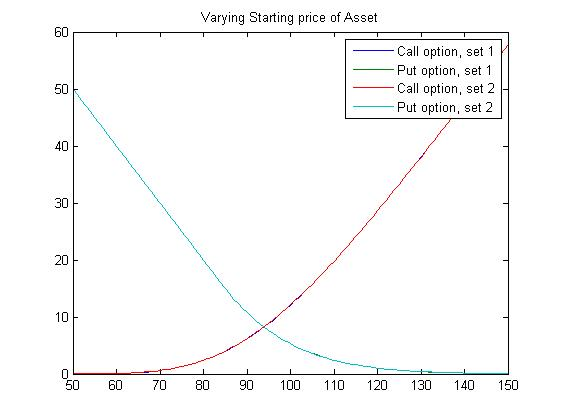
\includegraphics[width=6in]{start.jpg}
    \end{center}
        \subsubsection*{Dependence on Strike Price}
    \begin{center}
      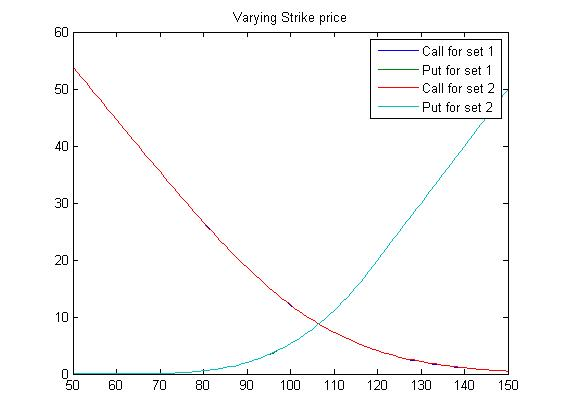
\includegraphics[width=6in]{strike.jpg}
    \end{center}
        \subsubsection*{Dependence on Rate}
    \begin{center}
      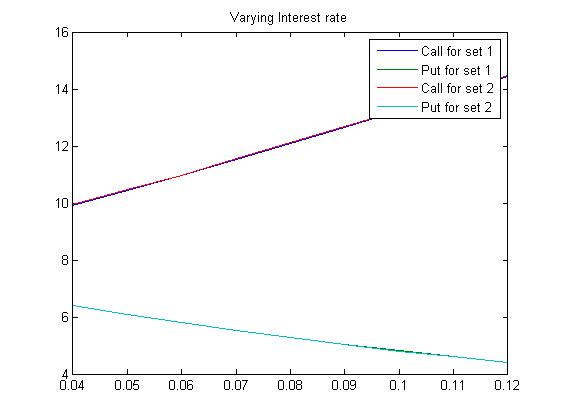
\includegraphics[width=6in]{rate.jpg}
    \end{center}
        \subsubsection*{Dependence on Volatility}
    \begin{center}
      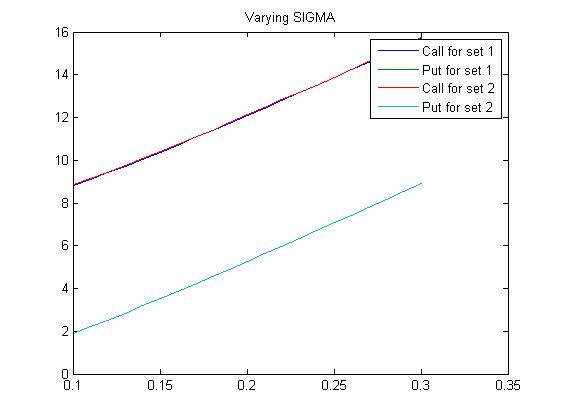
\includegraphics[width=6in]{sigma.jpg}
    \end{center}
    \subsubsection*{Dependence on Number of Steps}
    \begin{center}
      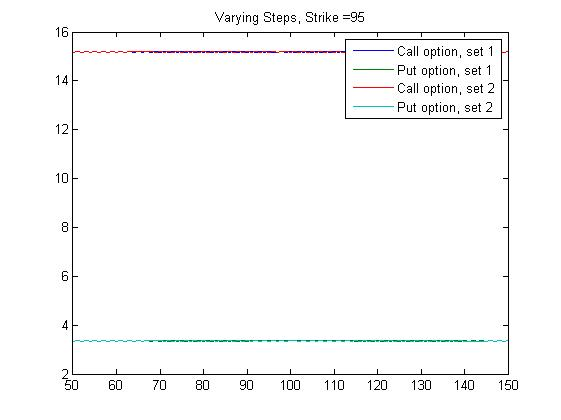
\includegraphics[width=6in]{steps95.jpg} \\
      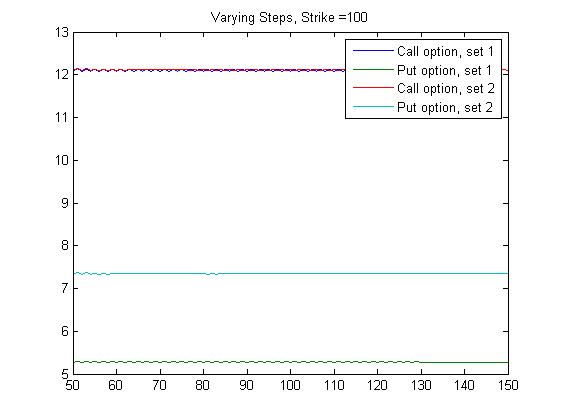
\includegraphics[width=6in]{steps100.jpg} \\
      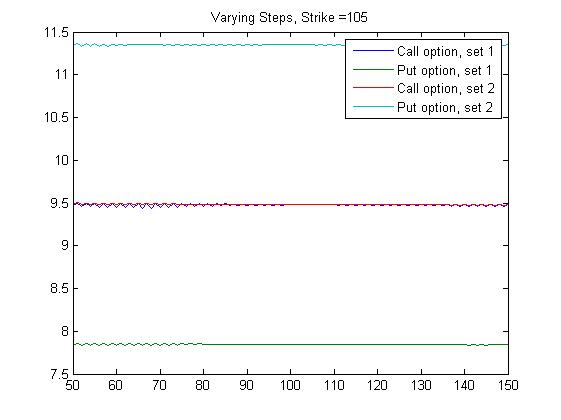
\includegraphics[width=6in]{steps105.jpg} \\
    \end{center}

\section{Question 2}
  \subsection*{Initial Prices of Lookback Put Option with Floating Strike}
    \begin{center}
    \begin{tabular}{c|c}
    M$\downarrow$ &Option price\\ \hline
    5 &9.1193\\
    10 &10.0806\\
    15 &10.5192\\ \hline
    \end{tabular}
    \end{center}
  \subsection*{Comparison}
    The value of option at time $t = 0$ increases with increasing steps; probably to converge to greater accuracy. Accurate conclusions cannot be drawn because the algorithm takes a long time to compute values for more time steps.


\newpage
\section{Code}
  \subsection*{Function for Valuating an American Call Option}
     \lstinputlisting{americancallWD.m}
  \subsection*{Function for Valuating an American Put Option}
     \lstinputlisting{americanputWD.m}
  \subsection*{Code for Analysing European Options}
     \lstinputlisting{lab3.m}
  \subsection*{Function for Valuating a Lookback Option}
     \lstinputlisting{lookback.m}


\end{document}